\documentclass[landscape]{article}
\usepackage{amsmath,amsthm,amsfonts,amssymb,amscd}
\usepackage{fullpage}
\usepackage{lastpage}
\usepackage{enumerate}
\usepackage{fancyhdr}
\usepackage[percent]{overpic}
\usepackage{mathrsfs}
\usepackage{wrapfig}
\usepackage{multirow}
\usepackage{amsmath}
\usepackage{url}
\usepackage{amssymb}
\usepackage{placeins}
\usepackage{amscd}
\usepackage{lscape}
\usepackage{graphicx}
\usepackage[usenames,dvipsnames]{color}
\usepackage{listings}
\usepackage[usenames,dvipsnames,svgnames,table]{xcolor}
\usepackage[left=2cm,right=2cm,top=2.5cm,bottom=2.5cm, headsep = 0.9cm]{geometry}
\usepackage{verbdef}
\setlength{\parindent}{0.0in}
\setlength{\parskip}{0.0in}
\usepackage{setspace}
\definecolor{gray}{RGB}{90,90,90}
\usepackage[colorlinks=true, linktoc=all, linkcolor=blue]{hyperref}
\usepackage{fancyvrb}
\usepackage{Sweave}
\usepackage{indentfirst}
\DefineVerbatimEnvironment{Sinput}{Verbatim} {xleftmargin=2em}
\DefineVerbatimEnvironment{Soutput}{Verbatim}{xleftmargin=2em}
\DefineVerbatimEnvironment{Scode}{Verbatim}{xleftmargin=2em}
\fvset{listparameters={\setlength{\topsep}{0pt}}}
\renewenvironment{Schunk}{\vspace{\topsep}}{\vspace{\topsep}}
\pagestyle{plain}
\setlength\parindent{1cm}

\begin{document}
\Sconcordance{concordance:test_cases.tex:test_cases.Rnw:%
1 37 1 1 4 11 1 1 2 4 0 1 2 4 1 1 2 1 0 5 1 3 0 1 2 1 1 1 2 4 0 1 2 5 1 1 2 1 0 1 1 3 0 1 2 14 1 1 2 21 0 1 2 1 1}

\centerline{\large{\textbf{Using \texttt{uwIntroStats}}}}
\centerline{\textbf{Authors: Brian D. Williamson and Scott S. Emerson, M.D., Ph.D.}}
\centerline{\textbf{University of Washington Department of Biostatistics}}
\tableofcontents
\newpage
\section{Introduction}

\section{Preparing \texttt{uwIntroStats}}


\indent Before we can dive in and run any analyses, we first need to install the package. This is done via
\begin{Schunk}
\begin{Sinput}
> install.packages("uwIntroStats")
\end{Sinput}
\end{Schunk}


Regardless of the graphical user interface (GUI) that you are using, R will prompt you to select a CRAN mirror. It is essentially asking you where you want to download the package files from. Select the mirror closest to you - for us at the University of Washington it is \texttt{WA(1)} or the Fred Hutchinson Cancer Research Center (FHCRC) - and the package will download and say that it has installed. Now each time we open a new R session (whether that is at the command line, a new RGui window, or a new RStudio window) we need to load the package for use. 

The \texttt{uwIntroStats} package relies on five other packages. These other packages provide key functions that the \texttt{uwIntroStats} package uses or adds functionality to. We must install these packages like we did above if we have not installed them previously, and then load \texttt{uwIntroStats}. While these packages do not need to be loaded every time (in fact, some are only used for specific functions) it is good practice to load them for the R session where you need to use \texttt{uwIntroStats}.
\begin{Schunk}
\begin{Sinput}
> library(Exact)
> library(geepack)
> library(plyr)
> library(sandwich)
> library(survival)
> library(uwIntroStats)
\end{Sinput}
\end{Schunk}

Don't worry about the warning message for now; that will be covered in section 3.2. Last, we load the data, \texttt{mri} that we will be using throughout this document. Information about the dataset can be found at \url{http://www.emersonstatistics.com/datasets/mri.pdf}. Since the data is part of the package, we can load it via
\begin{Schunk}
\begin{Sinput}
> data(mri)
\end{Sinput}
\end{Schunk}

The \texttt{uwIntroStats} package should be used for descriptive statistics, basic plotting (like scatterplots and boxplots), and regression analyses. The following sections will go through examples of these tasks, in addition to pointing out how our package differs from base R and other existing packages. We will assume familiarity with basic data manipulation and statistical tasks (for a refresher, see \url{http://www.emersonstatistics.com/GeneralMaterials/R/IntroToR.pdf}).

\section{Descriptive Statistics}
Descriptive statistics are an important part of any analysis. Often, they are just as important for the statistician or data analysist as they are for the scientific collaborators on a project. For example, descriptive statistics can help identify errors in the data, like observations that are particularly unusual (usually far out of the expected or observed range). They can also help to identify patterns of missing data, examine the study population, and identify aspects of the data that might lead to statistical issues. Descriptive statistics can also unearth relationships that had not previously been considered for analysis, thereby generating new studies. More information on this, and an outline of an approach to analysing a dataset, was written by Scott Emerson and can be found at \url{http://www.emersonstatistics.com/GeneralMaterials/analysis.pdf}. 

\subsection{The basics: \texttt{descrip()}}
The \texttt{uwIntroStats} package was designed with descriptive statistics in mind. The basic function for descriptive statistics is \texttt{descrip()}. This function takes in an arbitrary number of variables, and by default calculates the number of observations, the number of missing values, the mean, standard deviation, mininum value, maximum value, and the 25th, 50th, and 75th percentiles of each variable. For instance, if we wanted a quick glance at the \texttt{mri} data, we could type
\begin{Schunk}
\begin{Sinput}
> descrip(mri)
\end{Sinput}
\begin{Soutput}
            N     Msng  Mean      Std Dev    Min       25%       Mdn       75%       Max      
    ptid:     735     0   368.0     212.3     1.000     184.5     368.0     551.5      735.0  
 mridate:     735     0   76423     31896     10192     66642     80992     91392    1.232e+05
     age:     735     0   74.57     5.451     65.00     71.00     74.00     78.00      99.00  
    male:     735     0   0.4980    0.5003    0.0000    0.0000    0.0000    1.000      1.000  
    race:     735     0   1.318     0.6659    1.000     1.000     1.000     1.000      4.000  
  weight:     735     0   159.9     30.74     74.00     138.5     158.0     179.0      264.0  
  height:     735     0   165.8     9.710     139.0     158.0     165.9     173.2      190.5  
 packyrs:     735     1   19.60     27.11     0.0000    0.0000    6.500     33.75      240.0  
 yrsquit:     735     0   9.661     14.10     0.0000    0.0000    0.0000    18.50      56.00  
   alcoh:     735     0   2.109     4.852     0.0000    0.0000   0.01920    1.144      35.00  
 physact:     735     0   1.922     2.052     0.0000    0.5538    1.312     2.513      13.81  
     chf:     735     0  0.05578    0.2297    0.0000    0.0000    0.0000    0.0000     1.000  
     chd:     735     0   0.3347    0.6862    0.0000    0.0000    0.0000    0.0000     2.000  
  stroke:     735     0   0.2367    0.6207    0.0000    0.0000    0.0000    0.0000     2.000  
diabetes:     735     0   0.1075    0.3099    0.0000    0.0000    0.0000    0.0000     1.000  
 genhlth:     735     0   2.588     0.9382    1.000     2.000     3.000     3.000      5.000  
     ldl:     735    10   125.8     33.60     11.00     102.0     125.0     147.0      247.0  
     alb:     735     2   3.994     0.2690    3.200     3.800     4.000     4.200      5.000  
     crt:     735     2   1.064     0.3030    0.5000    0.9000    1.000     1.200      4.000  
     plt:     735     7   246.0     65.80     92.00     201.8     239.0     285.0      539.0  
     sbp:     735     0   131.1     19.66     78.00     118.0     130.0     142.0      210.0  
     aai:     735     9   1.103     0.1828    0.3171    1.027     1.112     1.207      1.728  
     fev:     735    10   2.207     0.6875    0.4083    1.745     2.158     2.649      4.471  
    dsst:     735    12   41.06     12.71     0.0000    32.00     40.00     50.00      82.00  
 atrophy:     735     0   35.98     12.92     5.000     27.00     35.00     44.00      84.00  
   whgrd:     735     1   2.007     1.410     0.0000    1.000     2.000     3.000      9.000  
  numinf:     735     0   0.6109    0.9895    0.0000    0.0000    0.0000    1.000      5.000  
  volinf:     735     1   3.223     17.36     0.0000    0.0000    0.0000   0.09420     197.0  
 obstime:     735     0    1804     392.3     68.00      1837      1879      2044      2159   
   death:     735     0   0.1810    0.3852    0.0000    0.0000    0.0000    0.0000     1.000  
\end{Soutput}
\end{Schunk}

This call gives us a quick look at the distribution of each variable in the sample, and can be easily exported to a word processing software. This is important, because displaying raw R output in a publication is not usually ideal, and taking the time to format the output is a pain.

Notice that there are a lot of variables measured in these data, and that some interesting phenomena are measured by multiple variables. For instance, smoking is measured by \texttt{packyrs} and \texttt{yrsquit} - if someone has zero pack-years (that is, they have never smoked) then they will also have zero years quit. Similarly, a current smoker of any amount of packs per year will have zero years quit. We can also look at the variables measured through blood samples, like LDL cholesterol (\texttt{ldl}) and get an idea of the range in our sample population. Last, in the variables like \texttt{male} which consist of only two values (sex was measured as male or female in this dataset), the mean tells us the proportion of our sample who was male (or for other binary variables, it will tell us the proportion which is coded as 1). The \texttt{descrip()} function works similarly to \texttt{summary()} in base R, but gives more information and returns it in a format that, as we described above, is easier to export from R.

Another powerful feature of \texttt{descrip()} is its ability to present stratified summaries, or summaries on a subset of the data. For instance, let's calculate descriptive statistics on the \texttt{age} variable within males and females:
\begin{Schunk}
\begin{Sinput}
> descrip(mri$age, strata = mri$male)
\end{Sinput}
\begin{Soutput}
                   N     Msng  Mean      Std Dev    Min       25%       Mdn       75%       Max     
mri$age:  All        735     0   74.57     5.451     65.00     71.00     74.00     78.00     99.00  
mri$age:    Str  0   369     0   74.41     5.258     65.00     71.00     73.00     78.00     91.00  
mri$age:    Str  1   366     0   74.73     5.642     66.00     71.00     74.00     78.00     99.00  
\end{Soutput}
\begin{Sinput}
> ## Call the summary function, to compare
> summary(mri$age)
\end{Sinput}
\begin{Soutput}
   Min. 1st Qu.  Median    Mean 3rd Qu.    Max. 
  65.00   71.00   74.00   74.57   78.00   99.00 
\end{Soutput}
\end{Schunk}

Here the row for \texttt{Str 0} corresponds to females (since they are coded as 0 for \texttt{male}), and males are \texttt{Str 1}. If we further wanted to restrict to only those people who were over 75 years old, we could use the \texttt{subset} argument:
\begin{Schunk}
\begin{Sinput}
> descrip(mri$age, strata = mri$male, subset = mri$age > 75)
\end{Sinput}
\begin{Soutput}
                   N     Msng  Mean      Std Dev    Min       25%       Mdn       75%       Max     
mri$age:  All        260     0   80.59     4.111     76.00     77.75     79.00     83.00     99.00  
mri$age:    Str  0   127     0   80.44     3.572     76.00     78.00     79.00     83.00     91.00  
mri$age:    Str  1   133     0   80.73     4.576     76.00     77.00     79.00     83.00     99.00  
\end{Soutput}
\end{Schunk}

However, the \texttt{descrip()} function can only give us a fixed number of summaries (mean, count, etc). Oftentimes we need only a subset of these, or perhaps different summary measures. For this, we turn to more powerful functions.

\subsection{Flexibility: \texttt{tableStat()} and \texttt{tabulate()}}
The main draw of \texttt{tableStat()} and \texttt{tabulate()} is their ability to supply only a subset of the summary measures from \texttt{descrip()}. These functions focus on display and flexibility. The user supplies the format for the summary statistics to be displayed in, which makes exporting results from a call to \texttt{tablestat()} or \texttt{tabulate()} even easier than it was for \texttt{descrip()}. Of the two, \texttt{tableStat()} is the base, and \texttt{tabulate()} adds some additional formatting and options. For example, let's say that we want the same summary statistics as we would get from \texttt{descrip()}, but we want to control the printout. For this, we use the \texttt{stat} argument. The options are presented in Table \ref{stattable}.
\begin{table}[ht]
\begin{tabular}{cl|cl}
Name & Summary Measure & Name & Summary Measure\\
\hline
\texttt{"count"} & Number of observations on a variable & \texttt{"sd"} & Standard Deviation\\
\texttt{"missing"} & Number of missing observations & \texttt{"variance"} & Variance\\
\texttt{"mean"} & Arithmetic mean & \texttt{"min"} & Minimum value\\
\texttt{"geometric mean"} & Geometric mean & \texttt{"max"} & Maximum value\\
\texttt{"median"} & 50th percentile & \texttt{"quantiles"} & Display quantiles\\
\texttt{"probabilities"} & Display percentiles & \texttt{"mn(sd)"} & Display Mean (SD) format\\
\texttt{"range"} & Maximum value - minimum value & \texttt{"iqr"} & Interquartile range (75th - 25th percentiles)\\
\texttt{"all"} & Display all summary measures & \texttt{"row\%"} & Display row percentages\\
\texttt{"col\%"} & Display column percentages & \texttt{"tot\%"} & Display percentage of total\\
\end{tabular}
\caption{Summary measures calculated by \texttt{tableStat()} and \texttt{tabulate()}.}
\label{stattable}
\end{table}
\FloatBarrier
The following gets us close to results we could display in a table for a puplication. We want to have 
\begin{displaymath}
N: \ n; \ Mean \ (SD): \ mn \ (sd); \ Range: \ max - min,
\end{displaymath}
which we get via:
\begin{Schunk}
\begin{Sinput}
> tableStat(mri$age, stat = "N: @count@; Mean (SD): @mean@ (@sd@); Range: @max@ - @min@")
\end{Sinput}
\begin{Soutput}
Tabled descriptive statistics by strata
Call:
      tableStat(variable = mri$age, stat = "N: @count@; Mean (SD): @mean@ (@sd@); Range: @max@ - @min@") 
            - NaN denotes strata with no observations
            - NA arises from missing or censored data

Format:  N: Cnt; Mean (SD): Mean (SD); Range: Max - Min 

                                                    .ALL 
N: 735.0; Mean (SD): 74.57 (5.451); Range: 99.00 - 65.00 
\end{Soutput}
\end{Schunk}

Note that all of the values enclosed in \texttt{@} symbols are from Table \ref{stattable} and are run by \texttt{tableStat()}, while the other values in the string are used for formatting. This function can also take stratification variables; if we want to see the above stratified by sex, we use
\begin{Schunk}
\begin{Sinput}
> tableStat(mri$age, strata = mri$male, stat = "N: @count@; Mean (SD): @mean@ (@sd@); Range: @min@ - @max@")
\end{Sinput}
\begin{Soutput}
Tabled descriptive statistics by strata
Call:
      tableStat(variable = mri$age, strata = mri$male, stat = "N: @count@; Mean (SD): @mean@ (@sd@); Range: @min@ - @max@") 
            - NaN denotes strata with no observations
            - NA arises from missing or censored data

Format:  N: Cnt; Mean (SD): Mean (SD); Range: Min - Max 

                                                strata.0                                                 strata.1                                               strata.ALL 
N: 369.0; Mean (SD): 74.41 (5.258); Range: 65.00 - 91.00 N: 366.0; Mean (SD): 74.73 (5.642); Range: 66.00 - 99.00 N: 735.0; Mean (SD): 74.57 (5.451); Range: 65.00 - 99.00 
\end{Soutput}
\end{Schunk}

Now if we wanted to see this in table form, in perhaps a nicer layout, we could use the \texttt{tabulate()} function. When we loaded the \texttt{uwIntroStats} package at the beginning of this document, recall that we got a warning message from R saying
\begin{verbatim}
The following object is masked from ‘package:base’:

    tabulate
\end{verbatim}

This means that our function \texttt{tabulate()} overwrites the function called \texttt{tabulatte()} in the base R package, which takes a numeric vector and counts the number of times each integer occurs in it. Our function does a similar task, but on combinations of strata. The syntax is very similar to the syntax for \texttt{tableStat()}, but rather than explicitly telling \texttt{tabulate()} the strata, it creates the tables with each dimension corresponding to a variable in the order they are entered. For instance, if we want a table of \texttt{age} (in the rows) and \texttt{male} (in the columns), we would write
\begin{Schunk}
\begin{Sinput}
> tabulate(mri$age, mri$male)
\end{Sinput}
\begin{Soutput}
Call:
tabulate(mri$age, mri$male)
            mri$male.0 mri$male.1 mri$male.ALL
mri$age.65    2          0          2         
mri$age.66    2          1          3         
mri$age.67   18         15         33         
mri$age.68   20         21         41         
mri$age.69   19         19         38         
mri$age.70   30         30         60         
mri$age.71   37         39         76         
mri$age.72   31         28         59         
mri$age.73   27         28         55         
mri$age.74   29         26         55         
mri$age.75   27         26         53         
mri$age.76   11         17         28         
mri$age.77   18         19         37         
mri$age.78   18         19         37         
mri$age.79   19         13         32         
mri$age.80    8         15         23         
mri$age.81   10         10         20         
mri$age.82   10          5         15         
mri$age.83   10          2         12         
mri$age.84    5          6         11         
mri$age.85    3          6          9         
mri$age.86    5          5         10         
mri$age.87    4          4          8         
mri$age.88    2          1          3         
mri$age.89    2          3          5         
mri$age.90    0          4          4         
mri$age.91    2          0          2         
mri$age.92    0          1          1         
mri$age.94    0          1          1         
mri$age.95    0          1          1         
mri$age.99    0          1          1         
mri$age.ALL 369        366        735         
            Point Estimate Test Statistic df 95% CI p-value Warnings
Chi-squared                26.244         30        0.66262         
\end{Soutput}
\end{Schunk}

By default, \texttt{tabulate} gives us the count in each combination of the strata, and gives us the overall $\chi^2$ test statistic, degrees of freedom, and p-value. We can add in other arguments as well. Let's say that we are interested in an odds ratio or a risk ratio - \texttt{tabulate()} can supply these, if we set \texttt{dispRatios = TRUE}. However, we supply both the odds ratio and the risk ratio, even though in some cases only one is appropriate. Thus it is up to the user to know which they can use. To display these ratios for \texttt{male} versus \texttt{chf} (an indicator variable of whether the patient had been diagnosed with congestive heart failure prior to MRI), we type
\begin{Schunk}
\begin{Sinput}
> tabulate(mri$male, mri$chf, dispRatios = TRUE)
\end{Sinput}
\begin{Soutput}
Call:
tabulate(mri$male, mri$chf, dispRatios = TRUE)
             mri$chf.0 mri$chf.1 mri$chf.ALL
mri$male.0   354        15       369        
mri$male.1   340        26       366        
mri$male.ALL 694        41       735        
            Point Estimate Test Statistic df 95% CI           p-value  Warnings
Chi-squared                3.2214         1                   0.072679         
Odds Ratio  1.8047                           [0.9396, 3.4663]                  
Risk Ratio  1.2944                           [1.0136, 1.6531]                  
\end{Soutput}
\end{Schunk}
Now we are given a point estimate and a 95\% confidence interval for both the odds and risk ratio, in addition to the $\chi^2$ estimate. 

Last, similar to \texttt{tableStat()}, we can identify different statistics to display. The syntax is exactly the same, and the same statistics from Table \ref{stattable} are valid in \texttt{tabulate()}.

\section{Plotting}
Plots and descriptive statistics together lead to a much better understanding of the data. In our package, we have implemented two types of plots: boxplots and scatterplots. In doing so, we have attempted to address some concerns with both types of plots.
\subsection{Boxplots}
Boxplots reduce the data down to four summary measures: minimum, maximum, median, and the interquartile range (25th to 75th quantile). They also show ``outliers'' in the data. We put this in quotes because the definition of ``outlier'' depends on the function you call, and the software you are running. Even in the base R version, \texttt{boxplot()}, the boxplots can be constructed so that no outliers are shown. 

Much of the criticism of boxplots lies both in this determination of outliers and in the dramatic reduction of the data. In our version, \texttt{bplot()}, we have added jittered data onto the boxplots (jittering allows us to see the data, but randomly adds noise so that we can see individual points better), and we have added the mean and standard deviation onto the plot. We can also produce stratified boxplots. For our function, the variable on the y-axis comes first, followed by the variable on the x-axis. This convention, while at odds with base R, is an attempt to make our functions match up with the regression scheme of response followed by predictors.

For our first example, let's create a boxplot showing the age distribution of the \texttt{diabetes} variable:
\begin{Schunk}
\begin{Sinput}
> ## Base R boxplot
> boxplot(mri$age ~ mri$diabetes)
> ## Our version of boxplot
> bplot(mri$age, mri$diabetes)
\end{Sinput}
\end{Schunk}
In comparing the two, see that our plot displays the mean line and $\pm$ standard deviation box in blue and overlays the jittered data on top of the boxplots produced by the base R function. Now if we also wanted to stratify by race, we write
\begin{Schunk}
\begin{Sinput}
> bplot(mri$age, mri$diabetes, strata = mri$race)
\end{Sinput}
\end{Schunk}
This boxplot breaks down diabetes by race, again showing the mean and standard deviation bars. Note that like normal plots, we can define the axis labels and title by hand.

\subsection{Scatterplots}
Scatterplots are a very common way to view data. They plot all of the data in one window, which allows the user to get a good overall view. However, many times the data is clumped together in some spots, and it is hard to see all of the points. Thus, similar to our approach in \texttt{bplot()}, our \texttt{scatter()} function jitters the data slightly by default. To illustrate this difference, we consider the distribution of cerebral atrophy by age group. In the base R scatterplot,
\begin{Schunk}
\begin{Sinput}
> plot(mri$age, mri$atrophy)
\end{Sinput}
\end{Schunk}
\begin{figure}[ht]
\begin{center}
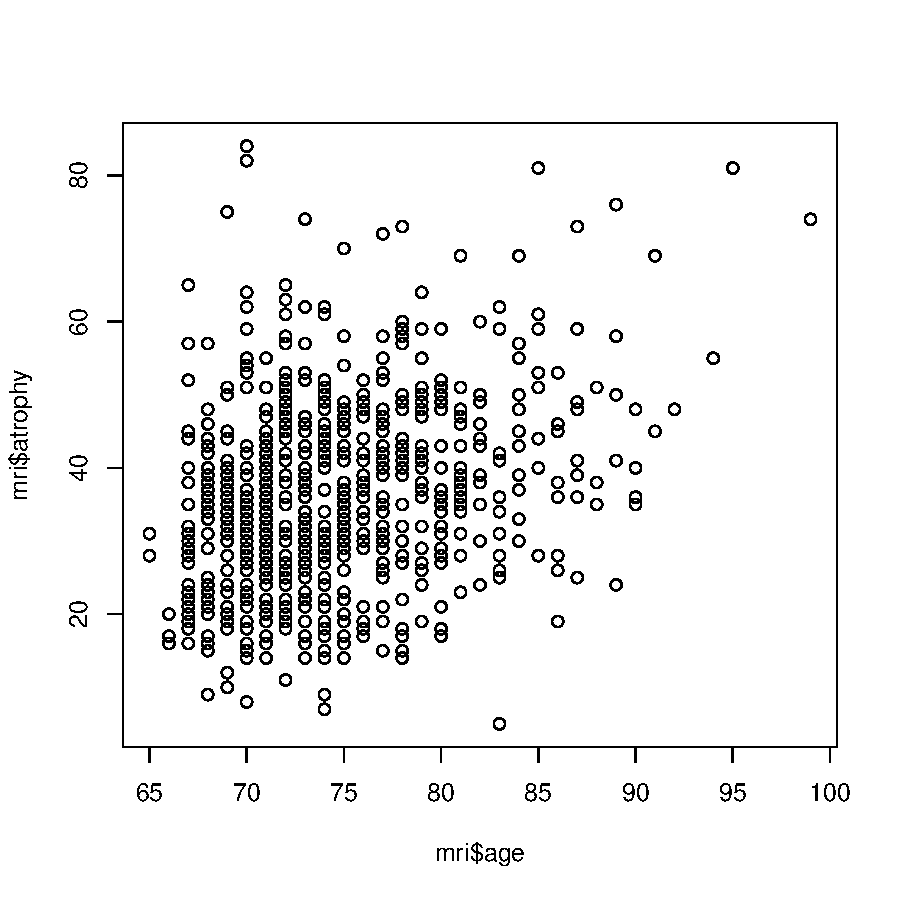
\includegraphics[width=0.4\textwidth]{test_cases-plot}
\caption{Base R Scatterplot}
\label{baseR}
\end{center}
\end{figure}
\FloatBarrier
we see that a lot of the values sit on top of each other. In our version (which again uses the Y followed by X convention),
\begin{Schunk}
\begin{Sinput}
> scatter(mri$atrophy, mri$age)
\end{Sinput}
\end{Schunk}
\begin{figure}[ht]
\begin{center}
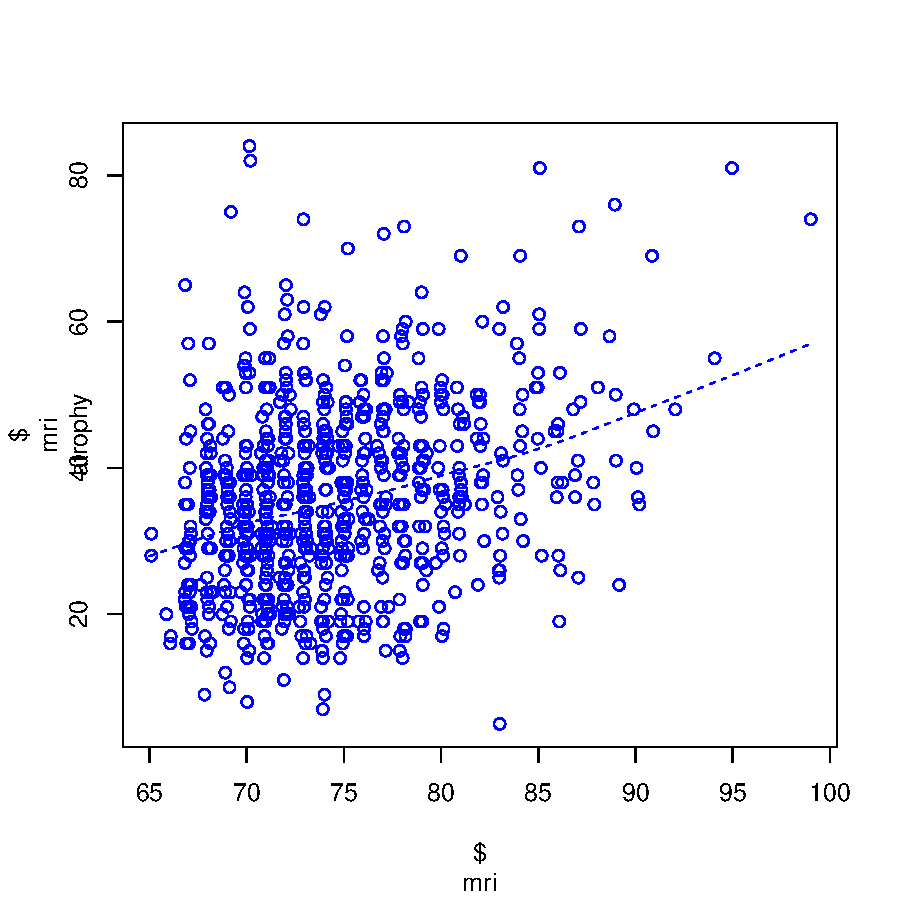
\includegraphics[keepaspectratio = true, width=0.4\textwidth]{test_cases-agescatter}
\caption{Scatterplot of atrophy vs age}
\label{agescatter}
\end{center}
\end{figure}
\FloatBarrier
the jittered data allows us to see where all of the points lie much better. Also notice that \texttt{scatter()} displayes a loess curve by default. We can also display a line of best fit calculated by least squares by adding \texttt{plotLSfit = TRUE}. Last, we can stratify, which is particularly useful if we want to see differences across a third variable, and \texttt{scatter()} will automatically color the data appropriately:
\begin{Schunk}
\begin{Sinput}
> scatter(mri$atrophy, mri$age, strata = mri$race)
\end{Sinput}
\end{Schunk}
\begin{figure}[ht]
\begin{center}
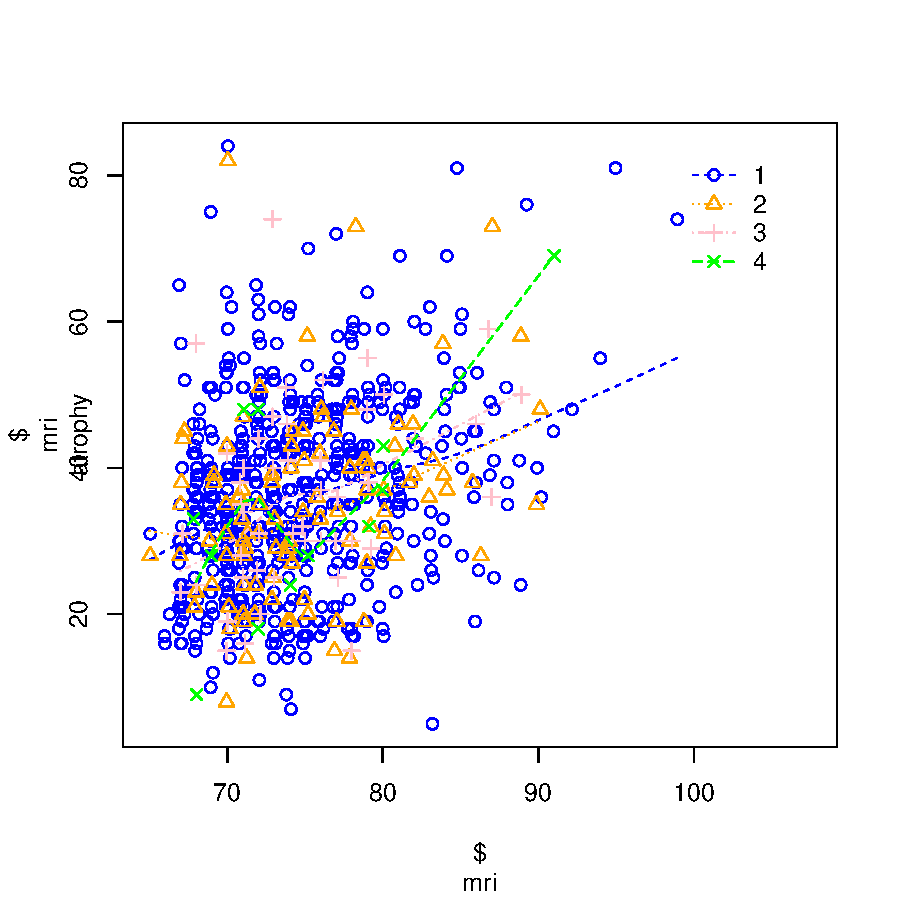
\includegraphics[keepaspectratio = true, width=0.4\textwidth]{test_cases-stratscatter}
\caption{Scatterplot of atrophy vs age stratified by race}
\label{stratscatter}
\end{center}
\end{figure}
\FloatBarrier

\section{Transformations of a Variable}
In many cases (especially in regression, which we will cover in section 7), it is more useful to model a transformation of a variable than the raw data itself. We present three functions to easily transform a variable. In each case, the function returns a list of: a matrix with the new transformed variable, the type of transformation performed, a vector describing how the variable was created, the name of the created variable, and the original data.
\subsection{Dummy Variables}
Dummy variables are a convenient way of creating indicator variables against some reference. For example, in the \texttt{mri} data, if we wanted to create a dummy variable for \texttt{race}, this would create 3 indicator variables (since there are four levels of race). By default, our \texttt{dummy()} function creates these indicators using the smallest value as the reference. 
\begin{Schunk}
\begin{Sinput}
> dummy.race <- dummy(mri$race)
> head(dummy.race, n = 10)
\end{Sinput}
\begin{Soutput}
      2 vs 1 3 vs 1 4 vs 1
 [1,]      1      0      0
 [2,]      1      0      0
 [3,]      1      0      0
 [4,]      0      0      0
 [5,]      0      0      0
 [6,]      0      0      1
 [7,]      0      0      0
 [8,]      1      0      0
 [9,]      0      0      0
[10,]      0      0      0
\end{Soutput}
\end{Schunk}
Thus the set of dummy variables for race created above has: an indicator of whether the patient is black or white, an indicator of whether the patient is Asian or white, and an indicator of whether the patient is listed as ``other'' or white. These variables would allow us, in a regression, to compare each of the races against the white reference group.

\subsection{Linear Splines}
Linear splines create a piecewise linear fit between user specified ``knot'' points; these are the points in the variable that we allow the slope of the line to change. There are two major ways to parameterize linear splines, and we have implemented both in this package. The first is based on the absolute slope between knots - that is, if we had a variable (like \texttt{ldl} in the \texttt{mri} dataset) that took on values between 11 and 247 and we placed knots at 70 and 150, we would see three columns: the first would show the minimum of 70 and the value of \texttt{ldl}; the second would show the minimum of \texttt{ldl} - 70 and 80; and the last column would show the remaining part of \texttt{ldl}. For example, if \texttt{ldl} = 71 for one patient, we would see \begin{verbatim} 70 1 0 \end{verbatim}. If \texttt{ldl} = 247, we would see \begin{verbatim} 70 80 97 \end{verbatim}.

The second parameterization is denoted by us as ``change''. This uses the change between knots to specify the slopes. Under this parameterization, we would see, for a value of 115, \begin{verbatim} 115 45 0 \end{verbatim}, which corresponds to: 115 units between the minimum and the value, 45 units between knot 1 (at 70) and the value, and zero units between knot 2 (at 150) and the value. We do not show negative units.

These two parameterizations can be accessed via
\begin{Schunk}
\begin{Sinput}
> lspline.ldl <- lspline(mri$ldl, knots = c(70, 150))
> head(lspline.ldl, n = 10)
\end{Sinput}
\begin{Soutput}
  $ mri ldl
 70  65   0
 70  14   0
 70  45   0
 61   0   0
 70  78   0
 70  80  13
 70  31   0
 70  46   0
 70  54   0
 70  40   0
\end{Soutput}
\begin{Sinput}
> lsplineD.ldl <- lsplineD(mri$ldl, knots = c(70, 150))
> head(lsplineD.ldl, n = 10)
\end{Sinput}
\begin{Soutput}
 x:min x: 70 x:150
   135    65     0
    84    14     0
   115    45     0
    61     0     0
   148    78     0
   163    93    13
   101    31     0
   116    46     0
   124    54     0
   110    40     0
\end{Soutput}
\end{Schunk}
\subsection{Polynomials}
Last we come to polynomials. This function creates a polynomial of the specified degree simply by multiplying the variable by itself the correct number of times. If we wanted to create a parabola in \texttt{age}, we type
\begin{Schunk}
\begin{Sinput}
> age.parabola <- polynomial(mri$age, degree = 2)
> head(age.parabola, n = 10)
\end{Sinput}
\begin{Soutput}
      Linear(ctr) Square(ctr)
 [1,]  -2.5659864   6.5842862
 [2,]   6.4340136  41.3965311
 [3,]  15.4340136 238.2087760
 [4,]  -2.5659864   6.5842862
 [5,]  -4.5659864  20.8482318
 [6,]  -2.5659864   6.5842862
 [7,]   0.4340136   0.1883678
 [8,]   0.4340136   0.1883678
 [9,]  -7.5659864  57.2441501
[10,]  -4.5659864  20.8482318
\end{Soutput}
\end{Schunk}
The ``(ctr)'' after each term tells us that \texttt{polynomial()} has automatically centered each term, and by default it centers at the mean of the variable. 

\section{One and Two Sample Functions}
Many of our analyses boil down to one-sample or two-sample problems; What is the mean time to death? What is the median home price in Seattle? What is the difference in mean time to death between control and the treatment group? The list goes on. There are many methods of analyzing one-sample relationships, and in our package we have implemented three. 
\subsection{Correlation}
While correlation is not an excellent source of inference, since it is inherently a feature of the dataset collected, sometimes it is important to know when variables are correlated. In the base R package, there are a few functions to calculate correlation: \texttt{cor()}, \texttt{var()}, \texttt{cov()}, and \texttt{cov2cor()}. Our function, \texttt{correlate()}, computes the correlation matrix between an arbitrary number of variables, and optionally also does this within a stratification variable. This is the real advantage of \texttt{correlate()}, since in base R we would have to manually subset the data into each stratum. If we want to examine the correlation between sex and diabetes, (and then stratify by race), we get
\begin{Schunk}
\begin{Sinput}
> ## Base R - returns only one number!
> cor(mri$male, mri$diabetes)
\end{Sinput}
\begin{Soutput}
[1] 0.1200211
\end{Soutput}
\begin{Sinput}
> ## uwIntroStats version
> correlate(mri$male, mri$diabetes)
\end{Sinput}
\begin{Soutput}
Tabled correlation statistics by strata
Call:
      correlate(mri$male, mri$diabetes) 
     Method:  Pearson 
     Data  :  Pairwise Complete 
            - NaN denotes strata with no observations
            - NA arises from missing data

##### ALL DATA
   ##  Estimated Correlation Coefficients 
                   mri$male:  mri$diabetes: 
    mri$male:  1.0000         0.1200        
mri$diabetes:  0.1200         1.0000        
\end{Soutput}
\begin{Sinput}
> ## Stratify on race
> correlate(mri$male, mri$diabetes, strata = mri$race)
\end{Sinput}
\begin{Soutput}
Tabled correlation statistics by strata
Call:
      correlate(mri$male, mri$diabetes, strata = mri$race) 
     Method:  Pearson 
     Data  :  Pairwise Complete 
            - NaN denotes strata with no observations
            - NA arises from missing data

##### Stratum   1 
   ##  Estimated Correlation Coefficients 
                   mri$male:  mri$diabetes: 
    mri$male:  1.0000         0.0941        
mri$diabetes:  0.0941         1.0000        

##### Stratum   2 
   ##  Estimated Correlation Coefficients 
                   mri$male:  mri$diabetes: 
    mri$male:  1.0000         0.2122        
mri$diabetes:  0.2122         1.0000        

##### Stratum   3 
   ##  Estimated Correlation Coefficients 
                   mri$male:  mri$diabetes: 
    mri$male:  1.0000         0.1155        
mri$diabetes:  0.1155         1.0000        

##### Stratum   4 
   ##  Estimated Correlation Coefficients 
                   mri$male:  mri$diabetes: 
    mri$male:  1.0000         0.3162        
mri$diabetes:  0.3162         1.0000        

##### ALL DATA
   ##  Estimated Correlation Coefficients 
                   mri$male:  mri$diabetes: 
    mri$male:  1.0000         0.1200        
mri$diabetes:  0.1200         1.0000        
\end{Soutput}
\end{Schunk}

Our function takes the pain out of calculating multiple correlations within stratum variables. We also return a correlation matrix rather than a single number, which allows the user to go straight to a covariance matrix by squaring. We also allow calculation of Spearman or Pearson (default) correlation.

\subsection{Point Estimates and Inference}
As mentioned above, since correlation is a function of the data gathered, we usually need other methods for our inference. One of the most common tests is the t-test, since we are often interested in the mean and making comparisons between means. Perhaps less common are the Wilcoxon and Mann-Whitney, which use the ``rank'' of the variables compared.   
\subsubsection{T-tests}
In the base R package, the \texttt{t.test()} function performs a t-test as you would expect. Our function \texttt{ttest()} improves on this by allowing stratification, calculation of the geometric mean, allowing for presuming unequal variances between samples, and making a cleaner output. For example, a t-test of whether the mean of the \texttt{ldl} variable is equal to 125 yields, in base R and \texttt{uwIntroStats}
\begin{Schunk}
\begin{Sinput}
> ## base R
> t.test(mri$ldl, mu = 125)
\end{Sinput}
\begin{Soutput}
	One Sample t-test

data:  mri$ldl
t = 0.64326, df = 724, p-value = 0.5203
alternative hypothesis: true mean is not equal to 125
95 percent confidence interval:
 123.3527 128.2528
sample estimates:
mean of x 
 125.8028 
\end{Soutput}
\begin{Sinput}
> ## uwIntroStats
> ttest(mri$ldl, null.hypoth = 125)
\end{Sinput}
\begin{Soutput}
Call:
ttest(var1 = mri$ldl, null.hypoth = 125)

One-sample t-test :
 
Summary:
 Variable Obs Missing Mean Std. Err. Std. Dev.     95% CI
  mri$ldl 735      10  126      1.25      33.6 [123, 128]

 Ho:  mean = 125 ; 
 Ha:  mean != 125 
 t = 0.6433 , df = 724 
 Pr(|T| > t) =  0.520256 
\end{Soutput}
\end{Schunk}

If instead we wanted a two-sample t-test of whether the difference in mean LDL between males and females were zero, we would get
\begin{Schunk}
\begin{Sinput}
> ## base R
> t.test(mri$ldl[mri$male == 0], mri$ldl[mri$male == 1])
\end{Sinput}
\begin{Soutput}
	Welch Two Sample t-test

data:  mri$ldl[mri$male == 0] and mri$ldl[mri$male == 1]
t = 4.1938, df = 721.23, p-value = 3.084e-05
alternative hypothesis: true difference in means is not equal to 0
95 percent confidence interval:
  5.502342 15.188221
sample estimates:
mean of x mean of y 
 130.9397  120.5944 
\end{Soutput}
\begin{Sinput}
> ## uwIntroStats
> ttest(mri$ldl, by = mri$male)
\end{Sinput}
\begin{Soutput}
Call:
ttest(var1 = mri$ldl, by = mri$male)

Two-sample t-test allowing for unequal variances :
 
Summary:
          Group Obs Missing  Mean Std. Err. Std. Dev.         95% CI
   mri$male = 1 369       4 130.9      1.79      34.3 [127.4, 134.5]
   mri$male = 0 366       6 120.6      1.69      32.1 [117.3, 123.9]
     Difference 735      10  10.3      2.47      <NA>    [5.5, 15.2]

 Ho: difference in  means = 0 ; 
 Ha: difference in  means != 0 
 t = 4.194 , df = 721 
 Pr(|T| > t) =  3.08428e-05 
\end{Soutput}
\end{Schunk}

Note that in our package, the default is to presume unequal variances between samples, which the authors believe to usually be the correct course. Also, we don't have to subset the data manually. We also run two-sided tests by default, but others can be specified.

\subsubsection{Generic Inference}
Until now, all of the methods in this section work on multiple samples. However, if we want to produce point estimates, interval estimates, and p-values for an arbitrary functional (mean, geometric mean, proportion, median, quantile, odds) of a variable, we can use the \texttt{oneSample()} function. Base R does not have a function which performs this general inference all in one spot. In the following tests, we will run one- and two-sample t-tests and an exact binomial test, all on the LDL variable. The t-tests run by \texttt{oneSample()} are an alternative to \texttt{ttest()} as described above. The output is not as verbose, but all of the information is the same:
\begin{Schunk}
\begin{Sinput}
> ## base R
> t.test(mri$ldl, mu = 125)
\end{Sinput}
\begin{Soutput}
	One Sample t-test

data:  mri$ldl
t = 0.64326, df = 724, p-value = 0.5203
alternative hypothesis: true mean is not equal to 125
95 percent confidence interval:
 123.3527 128.2528
sample estimates:
mean of x 
 125.8028 
\end{Soutput}
\begin{Sinput}
> ## ttest
> ttest(mri$ldl, null.hypoth = 125)
\end{Sinput}
\begin{Soutput}
Call:
ttest(var1 = mri$ldl, null.hypoth = 125)

One-sample t-test :
 
Summary:
 Variable Obs Missing Mean Std. Err. Std. Dev.     95% CI
  mri$ldl 735      10  126      1.25      33.6 [123, 128]

 Ho:  mean = 125 ; 
 Ha:  mean != 125 
 t = 0.6433 , df = 724 
 Pr(|T| > t) =  0.520256 
\end{Soutput}
\begin{Sinput}
> ## oneSample
> oneSample("mean", mri$ldl, null.hypothesis = 125)
\end{Sinput}
\begin{Soutput}
Hypothesis test of two-sided alternative that Mean <> 125 
Method: One sample t test 
10 observations deleted due to missing values
    n       Mean    95% CIlo  95% CIhi  Null Hyp   P two   
   725      125.8     123.4     128.3     125.0     0.5203 
\end{Soutput}
\end{Schunk}

However, the true flexibility of the \texttt{oneSample()} function comes into play when we ask about different functionals. If we want inference on the geometric mean (which might make sense since LDL is a biological variable that may exhibit extreme values due to illness), in base R or with \texttt{ttest()} we have to logarithmically transform our variable and then run the t-test. With \texttt{oneSample()}, we simply run on \texttt{"geometric mean"}:
\begin{Schunk}
\begin{Sinput}
> ## base R
> t.test(log(mri$ldl), mu = log(125))
\end{Sinput}
\begin{Soutput}
	One Sample t-test

data:  log(mri$ldl)
t = -3.0054, df = 724, p-value = 0.002744
alternative hypothesis: true mean is not equal to 4.828314
95 percent confidence interval:
 4.774290 4.816983
sample estimates:
mean of x 
 4.795636 
\end{Soutput}
\begin{Sinput}
> ## ttest
> ttest(log(mri$ldl), null.hypoth = log(125))
\end{Sinput}
\begin{Soutput}
Call:
ttest(var1 = log(mri$ldl), null.hypoth = log(125))

One-sample t-test :
 
Summary:
     Variable Obs Missing Mean Std. Err. Std. Dev.       95% CI
 log(mri$ldl) 735      10  4.8    0.0109     0.293 [4.77, 4.82]

 Ho:  mean = 4.8283137373023 ; 
 Ha:  mean != 4.8283137373023 
 t = -3.005 , df = 724 
 Pr(|T| > t) =  0.00274401 
\end{Soutput}
\begin{Sinput}
> ## oneSample
> oneSample("geometric mean", mri$ldl, null.hypothesis = 125)
\end{Sinput}
\begin{Soutput}
Hypothesis test of two-sided alternative that GeomMn <> 125 
Method: One sample t test on log transformed data 
10 observations deleted due to missing values
    n      GeomMn   95% CIlo  95% CIhi  Null Hyp   P two    
   725      121.0     118.4     123.6     125.0    2.744e-03
\end{Soutput}
\end{Schunk}

We can also compute an exact binomial test of the proportion of LDL values that are greater than 128:
\begin{Schunk}
\begin{Sinput}
> ## base R
> binom.test(sum(mri$ldl > 128, na.rm = TRUE), n = sum(!is.na(mri$ldl)))
\end{Sinput}
\begin{Soutput}
	Exact binomial test

data:  sum(mri$ldl > 128, na.rm = TRUE) and sum(!is.na(mri$ldl))
number of successes = 336, number of trials = 725, p-value = 0.05338
alternative hypothesis: true probability of success is not equal to 0.5
95 percent confidence interval:
 0.4266728 0.5005223
sample estimates:
probability of success 
             0.4634483 
\end{Soutput}
\begin{Sinput}
> ## oneSample
> oneSample("prop", mri$ldl > 128, null.hypothesis = 0.5)
\end{Sinput}
\begin{Soutput}
Hypothesis test of two-sided alternative that Pr(Event) <> 0.5 
Method: One sample inference for binomial proportions using exact distribution (LR ordering) 
10 observations deleted due to missing values
     n     Pr(Event) 95% CIlo  95% CIhi  Null Hyp    P two  
   725       0.4634    0.4267    0.5005    0.5000   0.05338 
\end{Soutput}
\begin{Sinput}
> oneSample("prop", mri$ldl, above = 128, null.hypothesis = 0.5)
\end{Sinput}
\begin{Soutput}
Hypothesis test of two-sided alternative that Pr>128 <> 0.5 
Method: One sample inference for binomial proportions using exact distribution (LR ordering) 
10 observations deleted due to missing values
    n      Pr>128   95% CIlo  95% CIhi  Null Hyp   P two   
   725      0.4634    0.4267    0.5005    0.5000   0.05338 
\end{Soutput}
\end{Schunk}

The syntax for \texttt{oneSample()} is much more intuitive; we simply enter that we want to test a proportion, and then give the logical value to test or specify the threshold. Also, rather than having to count successes, the total, and dealing with missing values by hand, we can let \texttt{oneSample()} handle everything for us and give output that is clearer to read.

\subsubsection{Wilcoxon and Mann-Whitney}
The most similar function between our package and the base R package is the function to perform Wilcoxon Signed Rank tests and Mann-Whitney-Wilcoxon Ranked Sum tests. Our function, \texttt{wilcoxon()}, adds formatting and variances, and prints the z-score and p-value in addition to the test statistic and p-value. Otherwise, the functions are the same, though we follow our usual syntax of Y followed by X. For example, if we want to test diseased versus healthy (in a made-up dataset), we can get 

\begin{Schunk}
\begin{Sinput}
> ## create the data
> cf <- c(1153, 1132, 1165, 1460, 1162, 1493, 1358, 1453, 1185, 1824, 1793, 1930, 2075)
> healthy <- c(996, 1080, 1182, 1452, 1634, 1619, 1140, 1123, 1113, 1463, 1632, 1614, 1836)
> ## base R
> wilcox.test(healthy, cf, paired = TRUE)
\end{Sinput}
\begin{Soutput}
	Wilcoxon signed rank test

data:  healthy and cf
V = 20, p-value = 0.08032
alternative hypothesis: true location shift is not equal to 0
\end{Soutput}
\begin{Sinput}
> ## uwIntroStats
> wilcoxon(cf, healthy, paired = TRUE)
\end{Sinput}
\begin{Soutput}
 Wilcoxon signed rank test 
         obs sum ranks expected
positive  10        71     45.5
negative   3        20     45.5
zero       0         0      0.0
all       13        91     91.0
                            
unadjusted variance   204.75
adjustment for ties     0.00
adjustment for zeroes   0.00
adjusted variance     204.75
                    H0 Ha       
Hypothesized Median 0  two.sided
  Test Statistic p-value 
V 71             0.080322
Z 1.7821         0.037368
\end{Soutput}
\end{Schunk}

Note that in the output of \texttt{wilcoxon()}, we have displayed the data calculated by the signed rank test, and given both the test statistic (V) and the z-score (Z).

\section{Regression}
Regression is one of the most widely used and easily understood methods of statistical analysis. The base R package has many different functions to perform regression: \texttt{lm()} for linear regression, \texttt{glm()} for generalized linear regression (which allows you to perform logistic regression, for example), \texttt{coxph()} for proportional hazards regression, and \texttt{geeglm()} as (one) method for correlated data regression. Each function has slightly different options, and remembering all of these is a chore. Part of the motivation for \texttt{regress()} is to alleviate this problem. This function provides one interface through which all types of regression can be performed. We also print the output from the regression in a much more understandable manner. Also, as we did in \texttt{ttest()}, we allow the user to calculate and use robust standard error estimates (using the Huber-White sandwich estimator), which adds flexibility. The \texttt{regress()} function does all of this while keeping the same formula syntax as its predecessors: \texttt{y~x1+x2*x3} still produces a linear model with coefficients for \texttt{x1}, \texttt{x2}, \texttt{x3}, and the interaction between \texttt{x2} and \texttt{x3}. The next four subsections deal with aspects of \texttt{regress()} in more detail.

\subsection{Basics of \texttt{regress()}}
The minimum we need to enter into \texttt{regress} is a functional, a formula, and a dataset. A functional takes an object and returns a value; for instance, the mean is a functional because it takes a distribution and returns the mean. The allowed functionals are displayed in Table \ref{fnctl}. Once we have a functional in mind (for now we choose the mean), we need to decide if we want to use robust standard error estimates. The default in \texttt{regress()} is to use these estimates, since we usually believe that the variances are not truly equal between groups compared in a regression analysis. The base R functions do presume equal variances between groups, which can lead to conservative (or anti-conservative) inference in some situations. The last change we have made to the usual regression output is displaying F-statistics rather than t-statistics for the test of each variable. We decided to use the F-distribution to make our results line up more easily with classical ANOVA tables. In most cases, the F-statistic is simply the square of the t-statistic. The inference is the same. To see \texttt{regress()} in action, consider testing the association between age and atrophy. The syntax for this computation is the same as that for any of the previous commands you might have used. 

\begin{Schunk}
\begin{Sinput}
> ## base R
> summary(lm(atrophy ~ age, data = mri))
\end{Sinput}
\begin{Soutput}
Call:
lm(formula = atrophy ~ age, data = mri)

Residuals:
    Min      1Q  Median      3Q     Max 
-36.870  -8.589  -0.870   7.666  51.203 

Coefficients:
             Estimate Std. Error t value Pr(>|t|)    
(Intercept) -16.06213    6.25619  -2.567   0.0104 *  
age           0.69798    0.08368   8.341 3.64e-16 ***
---
Signif. codes:  0 '***' 0.001 '**' 0.01 '*' 0.05 '.' 0.1 ' ' 1

Residual standard error: 12.36 on 733 degrees of freedom
Multiple R-squared:  0.08669,	Adjusted R-squared:  0.08545 
F-statistic: 69.58 on 1 and 733 DF,  p-value: 3.635e-16
\end{Soutput}
\begin{Sinput}
> ## uwIntroStats
> regress("mean", atrophy ~ age, data = mri)
\end{Sinput}
\begin{Soutput}
Call:
regress(fnctl = "mean", formula = atrophy ~ age, data = mri)

Residuals:
    Min      1Q  Median      3Q     Max 
-36.870  -8.589  -0.870   7.666  51.203 

Coefficients:
                 Estimate  Naive SE  Robust SE    95%L      95%H         F stat    df Pr(>F)   
[1] Intercept     -16.06     6.256     6.701       -29.22    -2.907           5.75 1    0.0168 
[2] age            0.6980   0.08368   0.09002       0.5213    0.8747         60.12 1  < 0.00005

Residual standard error: 12.36 on 733 degrees of freedom
Multiple R-squared:  0.08669,	Adjusted R-squared:  0.08545 
F-statistic: 60.12 on 1 and 733 DF,  p-value: 2.988e-14
\end{Soutput}
\end{Schunk}

Note that by default, our output is printed in a table, rather than having to call \texttt{summary.lm()}. The inference on the individual coefficients is different because we have used the F-distribution and are using robust standard error estimates, but we get approximately the same p-values. Also, the overall F-statistic is different in our version because we are using the robust standard error estimates. The numbers next to the coefficients tell us which to specify in any post-testing commands we run (see section 8).

\subsection{Regression on different functionals}
As mentioned above, part of the motivation for the \texttt{regress()} function was to have all types of regression in one function. Thus the other functionals we allow, and their corresponding commands in base R, are displayed in Table \ref{fnctl}. Note that we only display the options which lead to a certain type of regression, not the rest of the syntax.

\begin{table}[ht]
\centering
\begin{tabular}{c|l|l}
Functional & Type of Regression & Previous command (package)\\
\hline
\texttt{"mean"} & Linear Regression & \texttt{lm()} (stats - base R)\\
\texttt{"geometric mean"} & Linear Regression on logarithmically transformed Y & \texttt{lm()} ,with Y log transformed (stats - base R)\\
\texttt{"odds"} & Logistic Regression & \texttt{glm(family = binomial)} (stats - base R)\\
\texttt{"rate"} & Poisson Regression & \texttt{glm(family = poisson)} (stats - base R)\\
\texttt{"hazard"} & Proportional Hazards Regression & \texttt{coxph()} (survival)
\end{tabular}
\caption{Allowed functionals for \texttt{regress()}.}
\label{fnctl}
\end{table}
\FloatBarrier

If we enter a functional other than the mean, there is usually a transformation that needs to be applied to the data within the \texttt{regress()} function. In all of the cases listed in Table \ref{fnctl}, the transformation is the logarithm. For example, sometimes the logistic regression model is taught as having a ``log link'', or the poisson regression model is taught as having the ``logit link''. These both refer to the function of the parameter having logarithms, so that the model is linear in the coefficients on the predictors. Therefore, in each case, we back-transform - by using the \texttt{exp(x)} function, which is equivalent to $e^x$ - the output of the regression by default, but also display the output that has not been back-transformed. This allows the user to easily see the results in the correct units, while also retaining the ability to compare with other software or handle the un-exponentiated results. If we want to examine the association between LDL and age, but want to use the geometric mean, we get
\begin{Schunk}
\begin{Sinput}
> regress("geom", ldl ~ age, data = mri)
\end{Sinput}
\begin{Soutput}
( 10  cases deleted due to missing values)


Call:
regress(fnctl = "geom", formula = ldl ~ age, data = mri)

Residuals:
     Min       1Q   Median       3Q      Max 
-2.39512 -0.17020  0.03572  0.19342  0.70883 

Coefficients:

Raw Model:
                 Estimate   Naive SE   Robust SE        F stat    df Pr(>F)   
[1] Intercept       4.876     0.1494     0.1437           1150.70 1  < 0.00005
[2] age          -1.077e-03  1.999e-03  1.932e-03            0.31 1    0.5771 

Transformed Model:
                 e(Est)    e(95%L)   e(95%H)         F stat    df Pr(>F)   
[1] Intercept      131.1     98.87     173.8           1150.70 1  < 0.00005
[2] age            0.9989    0.9951    1.003              0.31 1    0.5771 

Residual standard error: 0.2929 on 723 degrees of freedom
  (10 observations deleted due to missingness)
Multiple R-squared:  0.0004018,	Adjusted R-squared:  -0.0009808 
F-statistic: 0.3112 on 1 and 723 DF,  p-value: 0.5771
\end{Soutput}
\end{Schunk}

In the transformed table, we do not display the standard error estimates, since they do not scale appropriately with the transformation. We could compare this to the base R function by log-transforming the \texttt{ldl} variable, running \texttt{lm()}, and back-transforming the results ourselves:
\begin{Schunk}
\begin{Sinput}
> ## transform the ldl variable
> logldl <- log(mri$ldl)
> ## create the model
> mod <- lm(logldl ~ age, data = mri)
> ## view the coefficients (untransformed)
> summary(mod)
\end{Sinput}
\begin{Soutput}
Call:
lm(formula = logldl ~ age, data = mri)

Residuals:
     Min       1Q   Median       3Q      Max 
-2.39512 -0.17020  0.03572  0.19342  0.70883 

Coefficients:
             Estimate Std. Error t value Pr(>|t|)    
(Intercept)  4.875983   0.149445  32.627   <2e-16 ***
age         -0.001077   0.001999  -0.539     0.59    
---
Signif. codes:  0 '***' 0.001 '**' 0.01 '*' 0.05 '.' 0.1 ' ' 1

Residual standard error: 0.2929 on 723 degrees of freedom
  (10 observations deleted due to missingness)
Multiple R-squared:  0.0004018,	Adjusted R-squared:  -0.0009808 
F-statistic: 0.2906 on 1 and 723 DF,  p-value: 0.59
\end{Soutput}
\begin{Sinput}
> ## back-transform the coefficients and CI
> mod.sum <- summary(mod)
> ## this gives the coefficients
> exp(mod.sum$coefficients[,1])
\end{Sinput}
\begin{Soutput}
(Intercept)         age 
131.1029250   0.9989231 
\end{Soutput}
\begin{Sinput}
> ## this gives the CI
> exp(mod.sum$coefficients[,1] - 1.96*mod.sum$coefficients[,2])
\end{Sinput}
\begin{Soutput}
(Intercept)         age 
 97.8143254   0.9950173 
\end{Soutput}
\begin{Sinput}
> exp(mod.sum$coefficients[,1] + 1.96*mod.sum$coefficients[,2])
\end{Sinput}
\begin{Soutput}
(Intercept)         age 
 175.720447    1.002844 
\end{Soutput}
\end{Schunk}

First, this is much more work, and requires thought for how to calculate the confidence interval - should we use the convenient approximation of 1.96, or should we use the \texttt{qnorm()} function? Second, we again lose the option of using robust standard error estimates. To use these, we would have to manually code a few more lines, which would increase the likelihood of a small mistake in the code. Our \texttt{regress()} function pulls all of this together in a simple format, leading to much fewer mistakes.

\subsection{Correlated data regression}
This section does not serve as a primer for when to account for correlated data in your regression model; rather, if you know that you have correlated data, it gives you a method to accounting for it. We will not use the \texttt{mri} data for this example. Instead, we will use the \texttt{salary} data, available at \url{http://www.emersonstatistics.com/datasets/salary.txt}. The documentation for this file is at \url{http://www.emersonstatistics.com/datasets/salary.doc}. These data deal with salaries at the University of Washington, and have multiple records on most participants. In fact, for any current faculty member in 1995 who had been employed by the university for more than one year, there were yearly records dating back to when the faculty member was hired. Thus by nature these data are correlated - in the simplest sense, we expect that the salary for a single faculty member will rise (or at least stay constant) each year. Therefore, we need to use the correlated data apparatus built into \texttt{regress()}. This functionality uses the \texttt{geeglm()} function from the package \texttt{geepack}, but frames the output consistently with the rest of the \texttt{regress()} options and uses the same syntax.

First, let's create the data:
\begin{Schunk}
\begin{Sinput}
> salary <- read.table("http://www.emersonstatistics.com/datasets/salary.txt", header = TRUE, stringsAsFactors = FALSE)
> salary$female <- ifelse(salary$sex == "F", 1, 0)
\end{Sinput}
\end{Schunk}
This code makes sure that the header in the text file is read as variable names, and that the string variables do not get converted to factor variables. We also create an indicator variable of whether the person is female or not. Next, suppose we are interested in the mean salary for females as opposed to males. Since raises are usually calculated as a percentage of current salary, and starting salaries can vary by year, we decide that the year in which a person started is important in determining their salary. For a more in-depth look at this thought process, see any document on determining potential confounding variables (for one, see parts of \url{http://www.emersonstatistics.com/GeneralMaterials/analysis.pdf}). By adding the \texttt{id} argument to \texttt{regress()}, we can account for the correlated data. In the \texttt{salary} dataset, the ID column is named \texttt{id}, and thus we have:
\begin{Schunk}
\begin{Sinput}
> ## adjusting for correlated data
> regress("mean",salary ~ female*year, id = id, data = salary)
\end{Sinput}
\begin{Soutput}
Call:
regress(fnctl = "mean", formula = salary ~ female * year, data = salary, 
    id = id)

Deviance Residuals: 
    Min       1Q   Median       3Q      Max  
-3727.9   -907.4   -230.0    719.2   7605.5  

Coefficients:
                   Estimate  Std Err   95%L         95%H         Wald      df Pr(>|W|) 
[1] Intercept       -17417     283.6    -17973       -16861        3771.66 1  < 0.00005
[2] female            4102     528.7      3065         5138          60.20 1  < 0.00005
[3] year             255.5     3.536     248.6        262.5        5222.05 1  < 0.00005
[4] female:year     -57.88     6.370    -70.36       -45.39          82.56 1  < 0.00005

 Estimated Scale Parameters: 
            Estimate  Std.err
(Intercept)  2024610 77997.57

 Correlation: Structure =  independence 

 Number of Clusters:  1597 

 Maximum Cluster Size:  20 
\end{Soutput}
\begin{Sinput}
> ## without adjusting
> regress("mean", salary ~ female*year, data = salary)
\end{Sinput}
\begin{Soutput}
Call:
regress(fnctl = "mean", formula = salary ~ female * year, data = salary)

Residuals:
    Min      1Q  Median      3Q     Max 
-3727.9  -907.4  -230.0   719.2  7605.5 

Coefficients:
                   Estimate  Naive SE  Robust SE    95%L      95%H         F stat    df Pr(>F)   
[1] Intercept       -17417     176.5     167.6       -17745    -17088       10802.86 1  < 0.00005
[2] female            4102     420.7     299.5         3515      4689         187.59 1  < 0.00005
[3] year             255.5     2.021     2.005        251.6     259.5       16235.87 1  < 0.00005
[4] female:year     -57.88     4.757     3.541       -64.82    -50.94         267.10 1  < 0.00005

Residual standard error: 1423 on 19788 degrees of freedom
Multiple R-squared:  0.487,	Adjusted R-squared:  0.4869 
F-statistic:  7166 on 3 and 19788 DF,  p-value: < 2.2e-16
\end{Soutput}
\end{Schunk}
Notice that we get some extra information in the output where we adjusted - we see that there are 1597 unique faculty members in the data, and that the longest we have data for is 20 years. Therefore treating the data as independent, like we do in the second call to \texttt{regress()}, will lead to invalid standard error estimates and therefore invalid confidence intervals and inference. 

\subsection{Multiple-partial F-tests}
The major added functionality that \texttt{regress()} brings to the table is the ability to perform multiple-partial F-tests. Some of these are done automatically when certain dummy variables, polynomial variables, or linear splines are entered - if created in a manner similar to our functions above. Others must be specified by the user, using a special function called \texttt{U()}.

As an example of the automatic multiple-partial F-test calculation, let's say we run a regression of atrophy on race, modeled as dummy variables. Recall from our work above that the dummy variables created by \texttt{race} have three levels, and each is in reference to the level coded as \texttt{white}. When we run this regression,
\begin{Schunk}
\begin{Sinput}
> regress("mean", atrophy ~ dummy(race), data = mri)
\end{Sinput}
\begin{Soutput}
Call:
regress(fnctl = "mean", formula = atrophy ~ dummy(race), data = mri)

Residuals:
    Min      1Q  Median      3Q     Max 
-31.243  -9.243  -0.462   7.757  47.757 

Coefficients:
                   Estimate  Naive SE  Robust SE    95%L      95%H         F stat    df Pr(>F)   
[1] Intercept        36.24     0.5408    0.5438       35.18     37.31        4441.94 1  < 0.00005
    dummy(race)                                                                 0.65 3    0.5832 
[2]    race.2       -1.781     1.379     1.334       -4.401     0.8381          1.78 1    0.1823 
[3]    race.3        0.2676    1.962     1.904       -3.470     4.005           0.02 1    0.8882 
[4]    race.4       -1.493     3.772     4.422       -10.17     7.189           0.11 1    0.7357 

 Dummy terms calculated from race, reference = 1 

Residual standard error: 12.93 on 731 degrees of freedom
Multiple R-squared:  0.002535,	Adjusted R-squared:  -0.001559 
F-statistic: 0.6499 on 3 and 731 DF,  p-value: 0.5832
\end{Soutput}
\end{Schunk}
notice that the coefficients for each dummy variable are presented in the usual way (though it is up to you to remember what \texttt{race.2} stands for). However, there is a new line above all of the dummy variable coefficients. First we see that this line does not get a coefficient number - that's because this line is only for the multiple partial F-test. Also, note that the regression coefficients are indented beneath it. This denotes that these dummy variables all belong to the same original variable (race). The test has three degrees of freedom, because there are three dummy variables that it is simultaneously testing. Recall that in an F-test, and in the t-test of normal linear regression in \texttt{lm()}, the null hypothesis for each of the p-values presented in the regression table is that the regression coefficient is equal to zero. The multiple partial F-test simulataneously tests that \emph{all three} coefficients are equal to zero. It allows us to declare tha there is no significant association between race and atrophy at the 0.05 level, since we have tested all race variables simultaneoudly and returned a p-value of 0.58. 

We also see that after the coefficients table, \texttt{regress()} tells us how the dummy variables were computed. 

Now for the user-defined multiple-partial F-tests, we need to be a bit careful. If entered in a call to \texttt{regress()}, the \texttt{U()} function takes in a formula, which can be named, and returns the specified multiple-partial F-test to the regression output. It also adds any new variables to the regression model. As an example of the \texttt{U()} function, if we wanted to add age and male to our model, and we wanted to have a multiple-partial F-test of these two variables, we could add
\begin{Schunk}
\begin{Sinput}
> U(~age + male)
\end{Sinput}
\end{Schunk}
to the model above. 
\begin{Schunk}
\begin{Sinput}
> regress("mean", atrophy ~ dummy(race) + U(~age + male), data = mri)
\end{Sinput}
\begin{Soutput}
Call:
regress(fnctl = "mean", formula = atrophy ~ dummy(race) + U(~age + 
    male), data = mri)

Residuals:
    Min      1Q  Median      3Q     Max 
-34.120  -8.331  -0.434   7.325  53.915 

Coefficients:
                     Estimate  Naive SE  Robust SE    95%L      95%H         F stat    df Pr(>F)   
[1] Intercept         -17.87     6.079     6.589       -30.81    -4.933           7.35 1    0.0068 
    dummy(race)                                                                   1.14 3    0.3315 
[2]    race.2         -2.109     1.280     1.246       -4.554     0.3370          2.87 1    0.0909 
[3]    race.3          0.2664    1.822     1.780       -3.228     3.761           0.02 1    0.8810 
[4]    race.4         -2.812     3.503     3.812       -10.30     4.671           0.54 1    0.4609 
    U(age + male)                                                                52.66 2  < 0.00005
[5]   age              0.6866   0.08134   0.08836       0.5132    0.8601         60.38 1  < 0.00005
[6]   male             5.988     0.8867    0.8895       4.242     7.734          45.32 1  < 0.00005

 Dummy terms calculated from race, reference = 1 

Residual standard error: 12 on 729 degrees of freedom
Multiple R-squared:  0.1439,	Adjusted R-squared:  0.138 
F-statistic: 21.32 on 5 and 729 DF,  p-value: < 2.2e-16
\end{Soutput}
\end{Schunk}
Note that again the multiple-partial F-test line is not a coefficient, but that the variables specified in the \texttt{U()} forumla are part of the regression model. If we wanted to make this output a bit more readable, we could give the second multiple-partial F-test a name by adding \texttt{testnm = } within our call to \texttt{U()}, before the formula.
\begin{Schunk}
\begin{Sinput}
> regress("mean", atrophy ~ dummy(race) + U(ma = ~age + male), data = mri)
\end{Sinput}
\begin{Soutput}
Call:
regress(fnctl = "mean", formula = atrophy ~ dummy(race) + U(ma = ~age + 
    male), data = mri)

Residuals:
    Min      1Q  Median      3Q     Max 
-34.120  -8.331  -0.434   7.325  53.915 

Coefficients:
                   Estimate  Naive SE  Robust SE    95%L      95%H         F stat    df Pr(>F)   
[1] Intercept       -17.87     6.079     6.589       -30.81    -4.933           7.35 1    0.0068 
    dummy(race)                                                                 1.14 3    0.3315 
[2]    race.2       -2.109     1.280     1.246       -4.554     0.3370          2.87 1    0.0909 
[3]    race.3        0.2664    1.822     1.780       -3.228     3.761           0.02 1    0.8810 
[4]    race.4       -2.812     3.503     3.812       -10.30     4.671           0.54 1    0.4609 
    ma                                                                         52.66 2  < 0.00005
[5]   age            0.6866   0.08134   0.08836       0.5132    0.8601         60.38 1  < 0.00005
[6]   male           5.988     0.8867    0.8895       4.242     7.734          45.32 1  < 0.00005

 Dummy terms calculated from race, reference = 1 

Residual standard error: 12 on 729 degrees of freedom
Multiple R-squared:  0.1439,	Adjusted R-squared:  0.138 
F-statistic: 21.32 on 5 and 729 DF,  p-value: < 2.2e-16
\end{Soutput}
\end{Schunk}

Other than the new name, the output is exactly the same as our original call. 

\section{Analysis/Post-testing}
After we have created a regression model and run the test, sometimes we want to check parts of our model. Usually, this comes in the form of an ANOVA table testing whether a combination of our coefficients are simultaneously equal to zero. As we saw in the previous section, \texttt{regress()} allows us to run these types of commands within the regression call. However, to check these results - or to avoid using \texttt{U()} within a call to \texttt{regress()} - we can use post-testing commands. 

Also, it is sometimes of interest to predict on a new data set. The object created by a call to \texttt{regress()} is like all other regression objects (from calls to \texttt{lm()}, \texttt{glm()}, etc) in that it allows predictions.

\subsection{Linear Combinations of Regression Coefficients}
A very useful function in STATA is the \texttt{lincom} function. This is a post-testing function which allows the user to specify a linear combination of the regression coefficients to simultaneously test. We have recreated this function in R, and it follows a similar syntax. Recall that the \texttt{regress()} function displayes a number next to each coefficient in the coefficients table. These numbers refer to the position of each variable in the call to \texttt{lincom()}. The default null hypothesis is that the linear combination is equal to zero.

This function can take either a vector or a matrix determining the linear combination to test. To have a better idea of how this works, we provide an example. In the previous section, when we introduced multiple-partial F-tests, we ran a regression of atrophy on race (modeled as dummy variables), male, and age. We can perform the same test using \texttt{lincom()}:
\begin{Schunk}
\begin{Sinput}
> ## get the model
> mod <- regress("mean", atrophy ~ dummy(race) + age + male, data = mri)
> ## get the test of age and male
> lincom(mod, comb = c(0,0,0,0,1,1))
\end{Sinput}
\begin{Soutput}
H0: 1*age+1*male   =  0 
Ha: 1*age+1*male  !=  0 
   Estimate   Std. Err.           T Pr(T > |t|)        95%L        95%H 
     6.6744      0.8942      7.4645      1.0000      4.9190      8.4299 
\end{Soutput}
\end{Schunk}
This test gives us the same inference as before - that the probability of seeing this event is extrememly small if the null hypothesis is true. Now in some cases we might be interested in combinations that aren't just the raw data. If we want, for example, twice the male coefficient, we can get this easily:
\begin{Schunk}
\begin{Sinput}
> lincom(mod, comb = c(0,0,0,0,1,2))
\end{Sinput}
\begin{Soutput}
H0: 1*age+2*male   =  0 
Ha: 1*age+2*male  !=  0 
   Estimate   Std. Err.           T Pr(T > |t|)        95%L        95%H 
    12.6622      1.7814      7.1079      1.0000      9.1649     16.1596 
\end{Soutput}
\end{Schunk}

\subsection{Prediction}
Prediction with a \texttt{uRegress} object (which is created by a call to \texttt{regress()}) follows the same syntax as prediction for any other regression object. Say we have split the mri data into a training and test set to learn our linear regression model on. First we set a seed, so that our random number generator will always start in the same place and we are guaranteed reproducible results.
\begin{Schunk}
\begin{Sinput}
> set.seed(47)
> samp <- sample(1:nrow(mri), nrow(mri)/2, replace = FALSE)
> mri.train <- mri[samp, ]
> mri.test <- mri[-samp,]
> modlm <- lm(atrophy ~ age + male + dummy(race), data = mri.train)
> modreg <- regress("mean", atrophy ~ age + male + dummy(race), data = mri.train)
> predslm <- predict(modlm, data = mri.test)
> predsreg <- predict(modreg, data = mri.test)
> head(predslm, n = 5)
\end{Sinput}
\begin{Soutput}
     719      275      559      603      420 
34.67201 46.44437 31.99498 38.41326 38.41326 
\end{Soutput}
\begin{Sinput}
> head(predsreg, n = 5)
\end{Sinput}
\begin{Soutput}
     719      275      559      603      420 
34.67201 46.44437 31.99498 38.41326 38.41326 
\end{Soutput}
\end{Schunk}

The above code reassures us that the predictions given on a \texttt{uRegress} object are the same as the predictions given on a \texttt{lm} object. The same is true for all of the other types of regression possible with \texttt{regress()}.

\section{Diagnostics}
Besides the other tools we have already covered that can double as diagnostic tools - scatterplots, boxplots - sometimes it is useful to look at residuals calculated from a regression model. Objects of class \texttt{uRegress}, like all other regression objects, have a function to extract residuals. The function we use is \texttt{uresiduals()}, which can return unstandardized, standardized, studentized, or jackknifed residuals. If we want the residuals from the model regressing age on ldl, it is easy to get both studentized and jackknifed residuals.
\begin{Schunk}
\begin{Sinput}
> ldlReg <- regress("mean", age ~ ldl, data = mri)
> student.resid <- uResiduals(ldlReg, "studentized")
> jack.resid <- uResiduals(ldlReg, "jackknife")
> head(student.resid, n = 5)
\end{Sinput}
\begin{Soutput}
         1          2          3          4          5 
-0.4676531  1.1641617  2.8293373 -0.5011149 -0.8294973 
\end{Soutput}
\begin{Sinput}
> head(jack.resid, n = 5)
\end{Sinput}
\begin{Soutput}
         1          2          3          4          5 
-0.4674003  1.1644483  2.8431637 -0.5008553 -0.8293181 
\end{Soutput}
\end{Schunk}

As with prediction, the residuals can be returned from any regression type allowed by \texttt{regress()}.
\end{document}
